
\section{User Feedback}

%\msb{What kind of user feedback have we gotten?} \geza{done}

User feedback for HabitLab has been generally positive. On the Chrome store for the browser version, there are 26 reviews, with an average rating of 4.5 stars, while on the Play store for the mobile version, there are 24 reviews, with an average rating of 4 stars. Users leave us feedback, both positive and negative, in a number of forms -- through feedback forms within the interface, as shown in Figure~\ref{fig:feedback_form}, by filing issues on GitHub, or sending emails. A complete list of feedback that users agreed to have publicly shared is in Appendix~\ref{ch:github}.

\begin{figure}
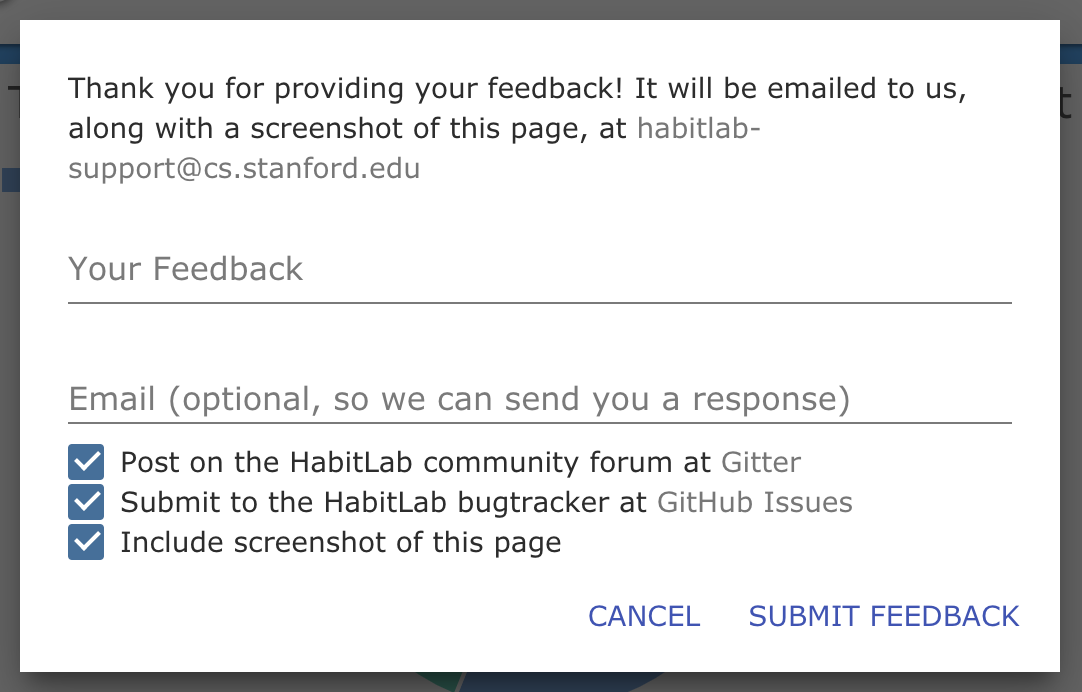
\includegraphics[width=\linewidth]{figuresS/feedback_form}
\caption{Our interface for submitting feedback within HabitLab.}
  \label{fig:feedback_form}
\end{figure}

%(Types of feedback and examples of them)

We find that most user feedback falls into the following categories:

\begin{itemize}
\item Requests:
\begin{itemize}
\item Requests for additional interventions
\item Requests for additional features and ways to customize the system
\item Requests for additional visualizations in the dashboard
\item Requests for site-specific functionality
\end{itemize}
\item Complaints:
\begin{itemize}
\item Complaints about resource usage
\item Complaints about particular interventions
\item Complaints about experience sampling
\item Complaints resulting from A/B testing and experimentation
\item Complaints due to user misunderstanding caused by excessive configurability
\end{itemize}
\item Positive feedback
\end{itemize}

\subsection{Requests}

\subsubsection{Requests for additional interventions}

We find that user feedback often request a specific intervention. Many are site-specific interventions. A commonly requested feature is to have combinations of interventions, or the ability to have multiple interventions active at once. We decided not to go down this path for two reasons:

\begin{itemize}
\item There is an exponential number of possible intervention combinations -- specifically, there are $2^n$ subsets of a group of n interventions. Thus, quantifying the effectiveness of combinations of interventions would take considerably more data than quantifying the effectiveness of individual interventions.
\item Some combinations of interventions would not work, provide a poor user experience, or would make little sense. For instance, it would make no sense to combine an intervention that injects items into feeds, with an intervention that removes feeds. To avoid deploying these to users, we would have to test and specify which particular subsets of interventions make sense to have together -- which, given that there an exponential number of possible intervention combinations, would take considerable effort.
\end{itemize}

Some examples of feedback of this form:

\textit{I think it would be great if there was the option for greater control to select multiple nudges to function every time. In my scenario, the website I want to control is Youtube. I use Youtube a lot whilst I'm working and being productive for various tutorials, downloading copyright fee assets and so on. However, the recommended videos often push click bait "trending" content at me, and having gone on Youtube to find a tutorial on solving a certain problem, you suddenly find your self 5 minutes into a "You won't BELIEVE what Gordan Ramsey says to this Chef" or similar rubbish. I'd really like to be able to use the Feed Diet, Sidekicker, Supervisor, and No Comment at the same time. I feel like your app has everything I need, but I can't use it all at the same time :)} -- \url{https://github.com/habitlab/habitlab/issues/641}

\textit{Youtube nudges not working as expected. Sidebar and comments turned on and showing normally. How many nudges can I active simultaneuosly?} -- \url{https://github.com/habitlab/habitlab/issues/620}

Users also often request new ideas for interventions. The following are some intervention ideas which were submitted via GitHub. The majority of ideas, however, are submitted via the idea voting interface in HabitLab, shown in Figure~\ref{fig:idea_voting} and are shown in Appendix~\ref{ch:ideas}.

\begin{figure}
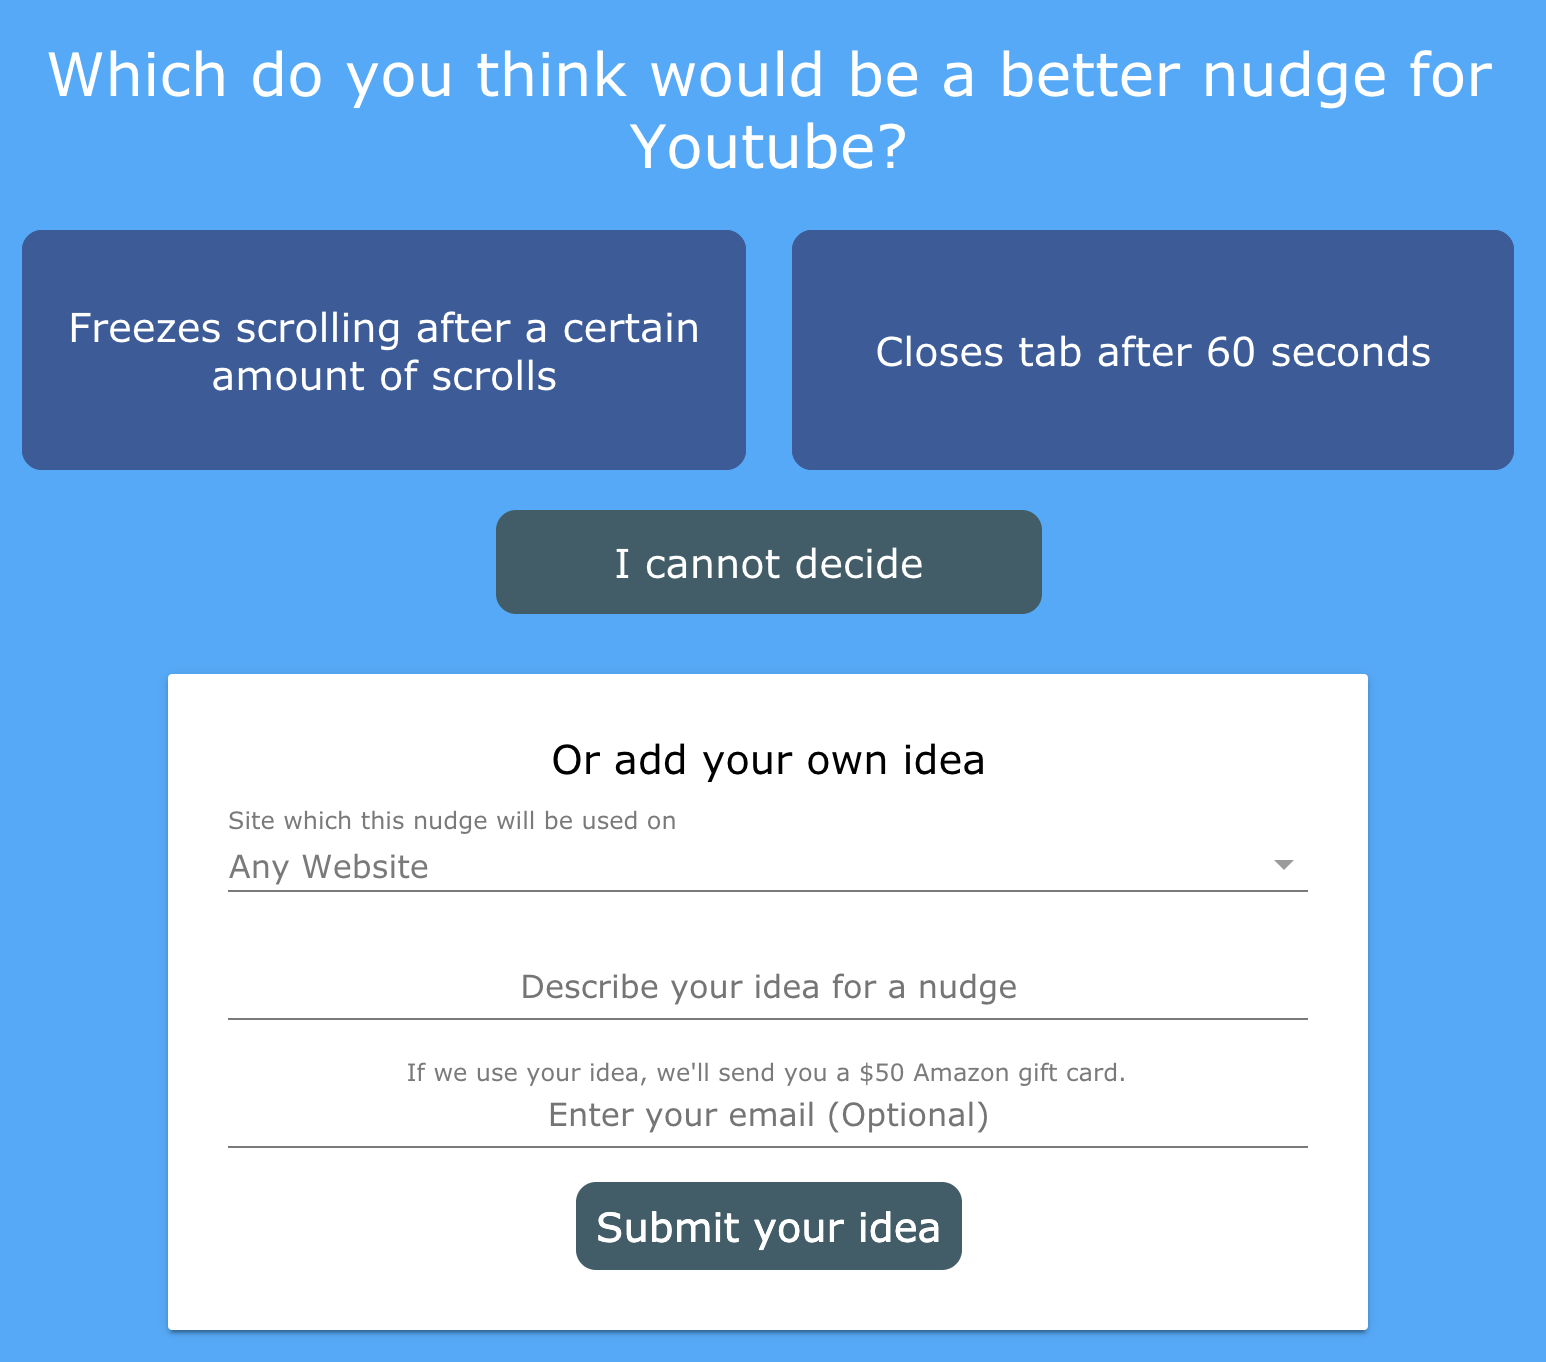
\includegraphics[width=\linewidth]{figuresS/idea_voting}
\caption{Our interface for letting users submit new intervention ideas and vote for existingones.}
  \label{fig:idea_voting}
\end{figure}

\textit{i would like to suggest maybe you can make another tracking nudge that only allows you to stay on a certain website and cant open any other tabs} -- \url{https://github.com/habitlab/habitlab/issues/593}

\textit{Hey! Would be nice to have displayed the total amount of time spent on the web. Great work, people! Thank you for making this :)} -- \url{https://github.com/habitlab/habitlab/issues/627}

\textit{Start making font (and other content) fade to grey with each scroll. Slowly the font will become tougher and tougher to read.} -- \url{https://github.com/habitlab/habitlab/issues/512}

\textit{nudge ``1 min assassin'' that decreases to e.g. 30sec assasin if you already spent 10 minutes on the domain} -- \url{https://github.com/habitlab/habitlab/issues/536}

\subsubsection{Requests for additional features and ways to customize the system}

Another commonly-seen request is for additional features and the ability to customize certain aspects of the program.

A commonly requested feature is the ability to turn off the ``Turn Off'' button which is present in each intervention.

\textit{Option to hide ``Turn off HabitLab'' button.} \url{https://github.com/habitlab/habitlab/issues/605}

\textit{Please add an option in settings to hide nudge turn off buttons (so they can only be turned off from settings page).} -- \url{https://github.com/habitlab/habitlab/issues/604}

\textit{Please allow option to not turn off buttons, e.g. "turn off feed eater button". Ideally this is a global option across all extensions. Thanks! :)} -- \url{https://github.com/habitlab/habitlab/issues/361}

Some users request more flexibility in which interventions are shown in particular contexts:

\textit{In general, I think the random is a good idea, but I quickly realize some of the random ones are ineffective for me. Rather than the random, it would be great if I could designate 1 feature for a particular website. For example, I know that facebook is a big time waster to me and moreso than others. I would love it if that was 1 one minute kick-off no matter what. Others (eg - Twitter) are less of a distraction for me, so the random wouldn't be as painful.} -- \url{https://github.com/habitlab/habitlab/issues/583}

\textit{have multiple slots for work times. eg : 8h00 12h00 and 14h00 18h00} -- \url{https://github.com/habitlab/habitlab/issues/533}

Some users request more flexibility in specifying sites to reduce time on, beyond our blacklist of domains model. One model frequently requested was a whitelist model:

\textit{I really wish there was a setting where I could use a nudge on every website except what's on a whitelist, because I always find a new place to waste time.} -- \url{https://github.com/habitlab/habitlab/issues/637}

\textit{Please add a whitelist for stricter management, so we add the sites we DO want to access.} -- \url{https://github.com/habitlab/habitlab/issues/548}

\textit{Can you make a whitelist version?} \url{https://github.com/habitlab/habitlab/issues/553}

Another model users suggested would be to group and categorize sites, and limit time across site categories:

\textit{You should be able to group sites and provide overall limits and timers across the category. For instance, Netflix and YouTube would be considered 'media streaming' allowing the user to set a goal of say an hour of streaming a day. Otherwise, I can personally see me spreading my viewing over multiple different websites to (pretend to) keep within the goals.} -- \url{https://github.com/habitlab/habitlab/issues/632}

Some users want more fine-grained ways to specify where to spend less time, beyond just the level of domains:

\textit{The extension doesn't track subdomains of a main domain properly. Suppose I add xyz.com as a filter and then it directs me to abc.xyz.com, the filter doesn't provide the needed nudges. This can be helpful if implemented.} -- \url{https://github.com/habitlab/habitlab/issues/566}

\textit{What about separating out Amazon from it's Kindle page (read.amazon.com) and it music page (music.amazon.com) because I enjoy listening to music when I type, and (sometimes) I read books on my Kindle from the website for work.} -- \url{https://github.com/habitlab/habitlab/issues/633}

\textit{On sites like news.google.com and reddit.com, you can click on links that take you to long articles on other domains where you can spend a significant chunk of time. Habit Lab doesn't track such changes now but really should!} -- \url{https://github.com/habitlab/habitlab/issues/601}

\textit{I want to be able to temporarily turn off nudges for a particular website. For example, I'm watching educational youtube videos, but still want to avoid other sites.} -- \url{https://github.com/habitlab/habitlab/issues/522}

\subsubsection{Request for additional visualizations in the dashboard}

Many users request additional information to be shown in the dashboard which we have the data for, but do not show any visualization for:

\textit{I would love it if it would give me a running tally of my total minutes spent in addition to the ``Today's five most visited sites by minutes spent'' Thanks and cheers!} -- \url{https://github.com/habitlab/habitlab/issues/562}

\textit{I want to see my history and detailed results for longer durations, such as weeks or months} -- \url{https://github.com/habitlab/habitlab/issues/618}

\textit{I want to see results per week and month - and to be able to compare each week / month. Also, an option to choose which day the week starts} -- \url{https://github.com/habitlab/habitlab/issues/597}

\textit{How much time did I spend on what tabs, last week? Where are the totals?} -- \url{https://github.com/habitlab/habitlab/issues/561}

\textit{Show total browsing time including those pages not in top 5.} -- \url{https://github.com/habitlab/habitlab/issues/607}

\subsubsection{Requests for site-specific functionality}

Other requests for features and customizations appear to be some specific to individual sites. Some examples are shown below:

\textit{Please let me have the ``Mission Objective'' nudge on youtube as well! I feel like it's one of the most effective nudges and would really make me consider twice whether to watch youtube or not.} -- \url{https://github.com/habitlab/habitlab/issues/544}

\textit{The disabling of autoplay makes me skip the recap of Jane The Virgin. However, that series includes new information and new jokes in every recap, so I always watch each recap even if I've just seen the previous episode. With autoplay on I can't watch the recap even if I've just logged in to Netflix, and even if I'm "rewinding" back to the beginning of the episode each time. It skips it again.} -- \url{https://github.com/habitlab/habitlab/issues/639}

\subsection{Complaints}

\subsubsection{Complaints about resource usage}

HabitLab is a complicated codebase with many background tasks, so it results in additional resource usage which may cause some users who monitor browser resources to uninstall it:

\textit{Disabling HabitLab due to excessive CPU usage. Right now the Chrome browser's TaskManage, CPU usage column shows HabitLab using 10-15\% CPU. Ouch! Adios!} -- \url{https://github.com/habitlab/habitlab/issues/634}

\textit{HabitLab extension in Chrome is using a lot of CPU} -- \url{https://github.com/habitlab/habitlab/issues/565}


\subsubsection{Complaints about particular interventions}

We have several complaints directed towards particular interventions. The more intrusive interventions, which may prevent the user from using some functionality on the site, in particular have more complaints directed towards them. Some examples of feedback of this form follow:

\textit{I came to Facebook to check notifications for events, but the scroll freezer hides the entire top bar. And the search bar too! I can't manage the events that I came here to manage. The other HabitLab stuff is good though!} -- \url{https://github.com/habitlab/habitlab/issues/617}

\textit{Nudges should NOT cover the page, they should possibly push the whole page down by the amount of space needed by the nudge. Most apps, like twitter and facebook, have their buttons at the top, and your nudges simply cover those and make the site unusable, so maybe one wants to do a quick action on the sites bar and leave, but the nudge bar is in the way, so one is forced to close the nudge to access the function of the site and get on with it. But then the nudge is closed} -- \url{https://github.com/habitlab/habitlab/issues/613}

\textit{Banner is too large} -- \url{https://github.com/habitlab/habitlab/issues/571}

\textit{I turned the restrict your time nudge off because it caps at 5 min. I like the idea, but it needs to be free form.} -- \url{https://github.com/habitlab/habitlab/issues/446}

\subsubsection{Complaints about experience sampling}

Experience sampling was a HabitLab feature that led to a number of complaints, despite our efforts to ensure they were as unintrusive as possible. Examples are shown below:

\textit{Whenever I go to a ``nudged site'', this ``how aggressive'' overlay comes up. I would not like it to. I click on ``Light touch'' every time, and it's so annoying that I'd sooner remove the Chrome extension than keep doing it every time. I get the thought, that maybe the annoyingness will make me visit those sites less. But if I wanted to not visit them at all, I'd just block them outright using another extension. I want to visit them, but be aware of how much time I'm spending. And I don't want additional tasks to accomplish every time. Would the "how aggressive" panel triggering-or-not be a setting you could add? I'd really like to keep using this system!} -- (via email)

\textit{How do I disable the ``How aggressive would you like HabitLab to be in helping you reduce your time spent this visit?'' message when going to Facebook? I find myself mindlessly clicking "don't do anything".... would prefer to have nudges on by default without an option to determine the strength BEFORE each FB visit ... this seems to be a new feature, that enables me to spend more time on FB without nudges ... how do I disable this??? TIA.} -- \url{https://www.reddit.com/r/habitlab/comments/a9kvly/how_do_i_disable_the_how_aggressive_would_you/}

\textit{it keeps asking me "how much do you want me to bother you??" and i am tired of answering this question. very cool extension that i used for like a year but something seems to have gone wrong so now i'm uninstalling :(} -- \url{https://github.com/habitlab/habitlab/issues/638}

\textit{Feed Eater Bug- if I have the feed eater feature enabled, every time I open facebook, there will be an alert window along the lines of "How aggressive would you like HabitLab to be in helping you reduce your time spent this visit?", which gets tiring when you have to open facebook a lot of times for personal matters (not time wasting stuff I swear). Update: Actually ignore what I just said about the Feed Eater bug, even with the feature off the issue continues on.} -- \url{https://github.com/habitlab/habitlab/issues/547}


\subsubsection{Complaints resulting from A/B tests and experimentation}

Some complaints were due to users misunderstanding how certain features of HabitLab work, which they perceived as being bugs.

One feature which frequently led to confusion was the rotating nature of interventions. Many users were expecting to see the same intervention every visit:

\textit{This is one of the most useful extensions when it comes to fighting web addiction. However, many of the nudges, such as the news eater for Facebook fail to work at some occasions. And most of them does not work when combined with other nudges. This often defeats the purpose of the extension entirely. Otherwise, I love the idea of having nudges, the pie chart for an overview and setting daily limits. In the meantime however, I will use News Feed Eradicator for Facebook, WasteNoTime and RescueTime instead.} -- \url{https://github.com/habitlab/habitlab/issues/511}

\textit{Sidekicker, and NoComments are not working on YouTube.com. They work on "Try now" mode, but when actually expecting it to run while browsing, it does not work. I can see see Comments and Side bar.} -- \url{https://github.com/habitlab/habitlab/issues/538}

\textit{Hello! I am not sure if I am understanding properly, but with the Bouncer nudge (my favourite), once you have done it once in a day it never triggers again. It would be good for it to ask every time I go to a site, how long I want to spend on it. And if I exit the site, it refreshes and starts again.} -- \url{https://github.com/habitlab/habitlab/issues/576}

Sometimes intentional artifacts of our A/B tests led users to believe that the system was broken or buggy. For example, in one of our A/B tests we varied the frequency at which interventions were shown, so often users would not see an intervention. This resulted in many users reporting bugs that they were not seeing interventions, even though this was intentional:

\textit{Why do I not always receive a nudge when I visit facebook, I keep compulsively checking, and hoping a nudge will remind me, but I don't seem to be seeing any.} -- \url{https://github.com/habitlab/habitlab/issues/557}

\textit{Nudges will frequently not show up when I visit facebook. Why is this? I haven't accidentally turned them off.} -- \url{https://github.com/habitlab/habitlab/issues/572}

\textit{the nudges arent really working....i have visited facebook multiple times now, but not have been nudged even once. I have enabled all the nudges as to see which one helps me the best, but its not nudging at all.} -- \url{https://github.com/habitlab/habitlab/issues/570}

\textit{None of the nudges are showing up. I'm not sure how to track down the issue. I've pasted the contents of the javascript console from a visit to YouTube here https://pastebin.com/ZyPYB2Tw in case it helps track down the issue. Does HabitLab not work alongside adblockers or ghostery or something like that?} -- \url{https://github.com/habitlab/habitlab/issues/569}

\textit{My nudges are not working most of time.} -- \url{https://github.com/habitlab/habitlab/issues/594}

\textit{It won't show nudges} -- \url{https://github.com/habitlab/habitlab/issues/585}

\subsubsection{Complaints due to user misunderstanding caused by excessive configurability}

Certain aspects of our system design caused user confusion and complaints. The most prominent ones were intervention rotation, and artifacts of A/B testing, which we described in separate sections above. Some others that resulted from a misunderstanding of functionality and controls are shown below:

Interventions are per-site, so if a user turns off an intervention on one site, it will not automatically turn off that intervention on other sites. This caused some users to believe that their request to turn off interventions was being ignored, when in reality they just had to turn it off on all sites. This suggests perhaps we should prompt the user whether they wish to turn off an intervention on all sites, when they disable it on one site, or simplify the configuration to default to turning interventions off on all sites by default:

\textit{I have told this app again and again that I want to turn off 2 nudges, freeze scrolling, and setting the number of minutes I want to spend on a website in advance. HOWEVER IT KEEPS COMING BACK and I am almost about to delete this despite loving ever other aspect of it. FIX THAT ASAP. OR don't say you can remove it if you can't.} -- \url{https://github.com/habitlab/habitlab/issues/628}

To satisfy various requests we received during development to be able to temporarily turn off interventions, we had options to turn off interventions for just that particular visit, for the entire day, or permanently. This sometimes led to confusion, as users would select the option to turn off an intervention temporarily, but they actually had intended to turn off the intervention permanently:

\textit{turned on for twitter - minute watch distracting / annoying, so turned on (?) "supervisor", turned off minute watch. It doesn't take. It still annoys. I'm about to simply turn off habit lab as a result.} -- \url{https://github.com/habitlab/habitlab/issues/522}

To address such confusion, We added some dialogs when turning off interventions to help explain what they would do, and provide alternative options in case they were looking to turn off interventions permanently or on all sites -- though this itself resulted in complaints:

\textit{When I turn off for the day/for the rest of the visit, it would be nice not to have a modal to confirm : I need one more click to close it, and it's annoying. If I wan't to turn it off, then there is no use anymore to slow down my use of thoses websites. See https://modalzmodalzmodalz.com/ for help} -- \url{https://github.com/habitlab/habitlab/issues/517}

Thus, user preferences are also extremely varied. In particular, users constantly request additional ways to customize and configure the system. However, if we add the ability to customize the system at too high a granularity, this may increase user confusion, as we observed with users intending to turn off an intervention permanently on all sites being frustrated that they were still seeing that intervention, once we added options to turn them off per-site or just temporarily that they mistook for turning them off permanently on all sites.

\subsection{Positive Feedback}

Some users also left us positive feedback:

\textit{Guys, I fuckingly love what you made! I send you all my gratitude for your wonderful product!} -- \url{https://github.com/habitlab/habitlab/issues/404}

\textit{YOU GUYS ARE AWESOME! I love nudges. I love Stanford. This helps me so much. I wish everybody knew about it.} -- \url{https://github.com/habitlab/habitlab/issues/406}
